\section{Le jeu de rôle, un renouveau de création populaire}

Le jeu de rôle est un style de jeu à travers lequel une personne incarne un personnage à travers lequel il agît dans un univers fictif. Ces jeux peuvent être réels (on parle alors de jeux de rôle grandeur nature, lorsqu'une personne joue physiquement un personnage de fiction), virtuels (jeux vidéos où le joueur contrôle un avatar) ou «sur table». Nous nous intéresserons ici à cette dernière catégorie, à laquelle se rapportera toute référence aux jeux de rôle dans la suite de cet écrit.

\subsection{Présentation JDR}

\begin{shadequote}
Le principe des jeux de role se rapproche davantage du théâtre improvisé que d'un jeu de société traditionnel. \par\emph{C{\'e}cile Cristofari \cite{cristofari2010lecteur}}
\end{shadequote}

%\begin{figure}[h!]
%    \centering
%    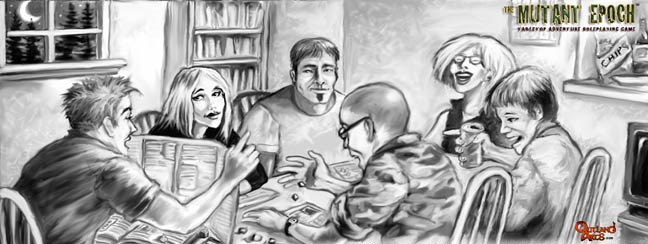
\includegraphics[width=0.80\linewidth]{img/rpg_tabletop1.jpg}
%    \caption{Tabletop RPG}
%\end{figure}


Jeu de société\\
Un Maître du jeu et entre trois et huit joueurs, chaque joueur interprétant un personnage imaginaire dont les dialogues et actions sont décrites à l'oral. Le maître du jeu, un narrateur, est en charge de choisir ou inventer un monde, une trame aventuresque contée, dans laquelle évolueront les joueurs. Il conte, décrit, fait survenir des évènements à sa convenance, devant également réagit aux actions des joueurs. Il s'agît pour les joueurs de résoudre des énigmes, combattre en équipe (mécanismes de dés afin d'évaluer la réussite d'une action) et vivre une expérience interactive reposant majoritairement sur l'imagination.\\
Une fois l'univers du jeu de rôle défini, les mécaniques du jeu doivent l'être. Il s'agît là de règles permettant d'évaluer la réussite des actions entreprises par les personnages joueurs et non joueurs, faisant souvent appels à des sets de dés dont le nombre de face varie usuellement de 4 à 20, l'interprétation des résultats dépendant en outre des caractéristiques des personnages concernées.\\
Un jeu de rôle n'a pour public que son maître du jeu et ses joueurs.\\
Le but d'une partie de jeu de rôle n'est pas tant de remporter la partie, le scénario de celle-ci pouvant être étendue avec pour seule limite la créativité du maître du jeu, mais plutôt de prendre plaisir à l'expérience imaginaire et sociale vécue. La partie, le plus souvent étalée sur plusieurs semaines, voire mois, prendra alors fin lorsque le maître du jeu estimera le monde suffisamment exploré, le scénario principal accompli ou par simple manque de temps. Il n'y a donc ni gagnant, ni perdant, le but étant la coopération des joueurs afin de vivre une aventure.\\

Les univers dont sont inspirés les mondes et scénarios ont souvent une origine littéraire (Call of Cthulhu, Lovecraft => ref, Le seigneur des anneaux, Tolkien) ou cinématographique (Star Wars).\\
La fidélité à l'oeuvre est alors libre au maître du jeu. On peut ainsi observer des fictions en accord irréprochable avec l'oeuvre dont elle sont issues, comme d'autres s'en inspirant vaguement, voire inventant un monde depuis ses fondements. Il en est de même pour le respect aux règles des jeux de rôles.\\
De nombreux livres de règles ont en effet été édités, chacun véhiculant avec lui la description étendue d'un monde, des races (humain, nain, elfe...) et classes (catégorie, telle magicien, prêtre, épéiste, chevalier...) de personnages, mais également des règles de jeu et un set de scénarios prédéfinis. Le respect de ces ouvrages est également laissé libre à chacun.\\

%\begin{figure}[h!]
%    \centering
%    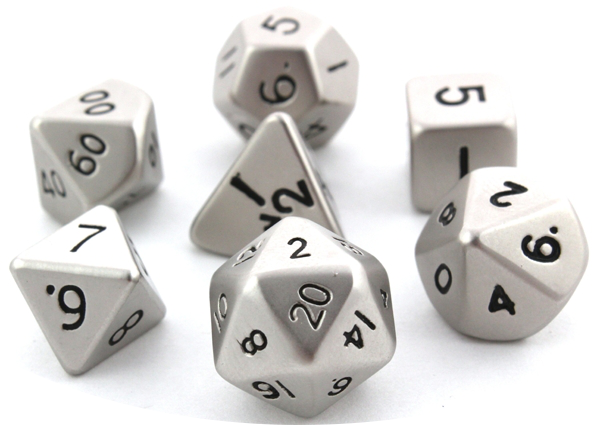
\includegraphics[width=0.80\linewidth]{img/dice_set.png}
%    \caption{Dice set}
%\end{figure}

\subsection{L'attrait des joueurs}
\begin{shadequote}
[...] il est important de s’identifier à un personnage qui permet de mettre en scène les désirs que le canon laisse insatisfaits [...]
\par\emph{C{\'e}cile Cristofari}
\end{shadequote}

L'attrait des joueurs pour les jeux de rôle proviet essentiellement de l'identification des joueurs au personnage que ceux-ci jouent, souvent plus importante que l'histoire vécue, pouvant entraîner une forte addiction, du même acabit que celle pouvant être constatée sur des jeux vidéos.

Le but du jeu de rôle est aussi d'étendre l'intrigue d'une oeuvre de fiction.

L'attrait des joueurs proviendrait selon Olivier Caïra\cite{caira2007jeux} de la multitude et de la complexité des compétences à mettre en oeuvre afin de pratiquer ce mode de jeu. Il s'agit en effet d'une cohabitation entre un maître du jeu et ses joueurs, ceux-ci devant effectuer une répartition des rôles au sein de leur équipe dans l'objectif d'augmenter leur efficacité à répondre aux évènements rencontrés par une complémentarité adéquate. Par ailleurs, la communication dont font preuve les joueurs se doit d'évoluer constamment, d'une part de par le niveau du registre de langue utilisé, mais également vis-à-vis de leur degré d'immersion dans le jeu (descriptions, commentaires hors du jeu, dialogues, précisions). Les joueurs doivent enfin faire preuve compétences variées (cohésion de groupe, éloquence, stratégie...) qui peuvent ici être perfectionnées.

Il s'agît en outre de vivre une autre vie, libéré des contraintes de la vie de tous les jours, désinhibé (voir partie suivante) et vivant le moi idéal

\subsection{Psychanalyse}
\begin{shadequote}
Le jeu de rôle en constitue un formidable outil qui visant à améliorer la communication, l'aisance sociale et la découverte de soi.
\par\emph{Anne-Marie Cariou-Rognant, Anne-Françoise Chaperon, Nicolas Duchesne, L'affirmation de soi par le jeu de rôle}
\end{shadequote}

Le jeu de role est en outre utilisé dans le domaine de la psychanalyse, considéré comme une aire d'expérience où les réactions de l'individu vis-à-vis de son environnement peuvent être analysées.

Étant bien souvent moins proche de la réalité que les contes, on peut y rencontrer davantage de stéréotypes, les joueurs choisissant souvent de s'idéaliser à travers le personnage joué afin d'obtenir dans ce monde imaginaire une place que ceux-ci ne parviennent pas à atteindre dans le monde réel.\\
Les joueurs peuvent aussi interpréter leur opposé (une personnalité extravertie pour un joueur timide, un fanatique religieux pour un athée). Ces jeux de rôles peuvent également être le lieu de réalisation de fantasmes et évènements socialement inacceptable dans le monde réel.

\clearpage
